\section{Design Overview}% 1-2pg}

% In this section, we present the overall design of our system and explain the
% structure of our policy synthesizer in detail.

\begin{figure}[tbp]
  \begin{tikzpicture}

    \node [draw,
      minimum width=2cm,
      minimum height=1.2cm,
    ]  (app) {Spring Web Applications};

    \node [draw,
      minimum width=2cm,
      minimum height=1.2cm,
      right=1.5cm of app,
    ]  (doop) {Doop};

    \node [draw,
      minimum width=2cm,
      minimum height=1.2cm,
      below=1cm of app,
    ]  (syn) {Policy Synthesizer};

    \node [draw,
      minimum width=2cm,
      minimum height=1.2cm,
      right=1.2cm of syn,
    ]  (detect) {Detect Vulnerabilities};

    \draw[-stealth] (app.east) -- (doop.west)
    node[midway,above]{*.jar file};

    \draw[-stealth] (app.south) -- (syn.north)
    node[midway,right]{API codes};

    \draw[-stealth] (doop.south) -- (syn.north)
    node[midway,right]{CallGraphEdge.csv};

    \draw[-stealth] (syn.east) -- (detect.west)
    node[midway,above]{Policies};

  \end{tikzpicture}
  \caption{System block diagram.}
  \label{fig:desgin}
\end{figure}

% \subsection{Overview}
Given a target spring web application (we chose lancie api here), we first used
Doop to do taint analysis on the target web application, which generates the
corresponding analysis file (e.g. CallGraphEdge.csv). We then designed and
implemented our security policy synthesizer that analyzes the taint analysis
output together with its API codes, to generate the security policies in our
designed format. In the end, we detected potential vulnerabilities by manually
analyzing the generated policies. The overall design of our workflow is shown as
Figure \ref{fig:desgin}.

The main work lies in the policy synthesizer design. We further separated it
into three steps: first, identify security-sensitive events by analyzing the
application codes; second, construct calling-context topology by analyzing the
Doop generated analysis file; and third, generate security policies by getting
the call-chain paths for all function calls that involve security-sensitive
events.

\section{Policy Synthesizer}
\label{sec:policy}

Our policy synthesizer takes the original API code together with analysis files
from Doop as inputs and outputs security policies for each of the API in the
spring web application.
%
This section describes our algorithm to generate security policies.
%

\subsection{Security-Sensitive Events Identification}
To generate security policies, it is important to first define what are the
security vulnerabilities, and recognize those security-sensitive events. There
are many types of possible security problems, including data safety,
authorization control, etc. In this project, we consider all operations that may
affect the integrity of database to be security-sensitive events, which includes
queries that insert, delete, or update the database.

By analyzing the API codes of this specific code repository, we concluded that
all the database related class are implemented from spring interface
\textit{JpaRepository} \footnote{Publicly available at:
  \url{https://docs.spring.io/spring-data/jpa/docs/current/api/org/springframework/data/jpa/repository/JpaRepository.html}.},
and end with name \textit{Repository}. By analyzing the available methods in
JpaRepository, we treated all methods that start with \textit{save} and
\textit{delete} as operations that will potentially modify the database. To
conclude, we treat all statements that conform to regex expression
\textit{$*$Repository.save$*$} or \textit{$*$Repository.delete$*$} as those
could affect the integrity of the database. After locating these
security-sensitive statements, we wrote a script to extract their corresponding
class and method names, and output in the format of
\textit{className:methodName(arguments...) $\rightarrow$ return type}, same as
the Doop generated analysis file format. These security-sensitive methods later
serve as the root for finding functions that involve security-sensitive events.


\subsection{Calling-Context Topology Construction}

\begin{figure}[tbp]
  \centering
  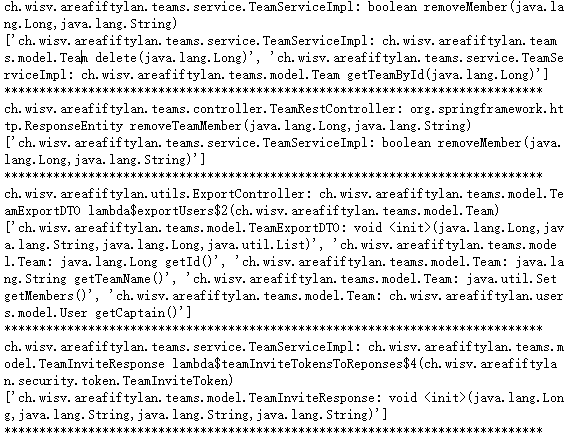
\includegraphics[width=0.48\textwidth]{img/caller2callee.png}
  \caption{Examples of three callers and lists of corresponding callees}
  \label{caller2callee}
\end{figure}

After identifying security-sensitive events, we build a topo graph of contexts
who start from those events, and end at program entry points. In our case, we
used Doop to make taint analysis on lancie api, which generates the many
analysis files, including \textit{CallGraphEdge.csv}. Caller function
information can be extracted from the second column of
\textit{CallGraphEdge.csv}, and information of a callee function that is called
by the caller can be extracted from the forth column. One caller has multiple
callees, and one calee might be called by multiple callers. To be notice, there
is no recursion functions, so the call graph is actually a topology. Figure
\ref{caller2callee} are some examples of three callers and lists of their
callees. The topo call graph is represented in the form of two Python
dictionaries. The keys of the first dictionary, \textit{parent2children}, are
callers, and values are lists of callees. On the other hand, the keys of the
second dictionary \textit{child2parents} are callees and values are lists of
callers.


\subsection{Security Policy Generation}

\begin{figure} [btp]
  \small
  \begin{tabular}{rcp{5cm}}
    Policy \hspace*{-3ex}    & $\rightarrow$ & \hspace*{-3ex} Statement$*$                                                      \\
    Statement \hspace*{-3ex} & $\rightarrow$ & \hspace*{-3ex} (Principal, Action, Resource)                                     \\
    Principal \hspace*{-3ex} & $\rightarrow$ & \hspace*{-3ex} Role $|$ Role(Condition) $|$ IsAuthenticated                      \\
    Role \hspace*{-3ex}      & $\rightarrow$ & \hspace*{-3ex} ROLE\_ADMIN $|$ ROLE\_OPERATOR $|$ ROLE\_COMMITTEE $|$ ROLE\_USER \\
    Condition \hspace*{-3ex} & $\rightarrow$ & \hspace*{-3ex} string$*$                                                         \\
    Action \hspace*{-3ex}    & $\rightarrow$ & \hspace*{-3ex} string$*$                                                         \\
    Resource \hspace*{-3ex}  & $\rightarrow$ & \hspace*{-3ex} string$*$                                                         \\
  \end{tabular}
  \caption{Simplified abstract syntax for our designed policy language}
  \label{fig:dsl}
\end{figure}

We define our policy language in a simplified abstract syntax.
%
We take inspiration from the simplified abstract
syntax~\cite{Backes+etal:2018:policy} defined for AWS and shows the abstract
syntax for our designed policy language in \fref{fig:dsl}.
%
In this syntax, $*$ denotes a list of valued elements.
%
A policy consists of a list of statements.
%
Each statement is a tuple that contains three elements: principal, action, and
resource.
%
The principal construct is used to specify users with which role or under
certain condition are granted access to the action and resource.
%
The action construct specifies the list of actions that are allowed to be
performed on the corresponding resource.
%
The resource construct specifies the list of resources in which access is
granted.

To generate policies for each API in the web application, we compute a set of
security-sensitive events and construct a calling-context graph.
%
For each API in the web application, we find all the call-chain path from the
API to security-sensitive events we detected in the calling-context graph.
%
Each call-chain path is one policy for the API.
%
Principal is obtained from the preAuthorize condition defined by the application
for the API.
%
We created a table to convert the condition in preAuthorize to Principal.
%
Action is defined as the method name fo the corresponding security-sensitive
event appeared on the path.
%
Resource is defined as the return type of the security-sensitive event function.
